\section{Non-Targeted and Targeted Attacks}

    \subsection{Non-Targeted Attacks}
        The idea is to generate some image that is designed to make the neural network have a certain output. For instance, say our goal label/output is $[0, 0, 0, 0, 0, 1, 0, 0, 0, 0]$.

        That is, we want to come up with an image such that the neural network’s output is the above vector. In other words, find an image such that the neural network thinks the image is a $5$ (remember, we’re zero indexing). It turns out we can formulate this as an optimization problem in much the same way we train a network. Let’s call the image we want to make $\overrightarrow{x}$ (a $784$ dimensional vector, because we flatten out the $28 \times 28$ pixel image to make calculations easier). We’ll define a cost function as $$ C = \frac{1}{2} \Vert y_{goal} - \hat{y}(\overrightarrow{x}) \Vert_{2}^{2} $$

        Where the $y_{goal}$ is our goal label from above. The output of the neural network given our image is $ hat{y}(\overrightarrow{x})$. You can see that if the output of the network given our generated image $\overrightarrow{x}$ is very close to our goal label $ y_{goal}$, then the corresponding cost is low. If the output of the network is very far from our goal then the cost is high. Therefore, finding a vector $\overrightarrow{x}$ that minimizes the cost CC results in an image that the neural network predicts as our goal label. Our problem now is to find this vector $\overrightarrow{x}$. \Cref{fig:non_targeted} shows one of the adversarial image generated by using back propagation with above specified cost function.

        \begin{figure}[htbp]
            \centering
                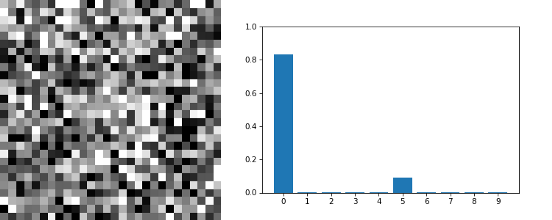
\includegraphics[width=0.7\linewidth]{images/non_targeted1.png}
            \caption{The left side is the non-targeted adversarial exampele (a 28 X 28 pixel image). The right side plots the activations of the network when given the image.}
            \label{fig:non_targeted}
        \end{figure}

    \subsection{Targeted Attacks}
        These adversarial examples are cool and all, but to humans they just look like noise. Wouldn’t it be cool if we could have adversarial examples that actually looked like something? Maybe an image of a $2$ that a neural network thought was a $5$? It turns out that’s possible! And moreover, with just a very small modification to our original code. What we can do is add a term to the cost function that we’re minimizing. Our new cost function will be $$ C = \frac{1}{2} \Vert y_{goal} - \hat{y}(\overrightarrow{x}) \Vert_{2}^{2}  + \lambda \Vert  \overrightarrow{x} - x_{target}  \Vert_{2}^{2}   $$

        Where $x_{target}$ is what we want our adversarial example to look like ($x_{target}$ is therefore a $784$ dimensional vector, the same dimension as our input). So what we’re doing now is we’re simultaneously minimizing two terms. The left term we’ve seen already. Minimizing this will make the neural network output ygoalygoal when given $(\overrightarrow{x}$. Minimizing the second term will try to force our adversarial image x to be as close as possible to $x_{target}$ as possible (because the norm is smaller when the two vectors are closer), which is what we want! The extra $\lambda$ out front is a hyperparameter that dictates which of the terms is more important. As with most hyperparameters I find after a lot of trial and error that $.05$ is a good number to set $\lambda$ to. If you know about ridge regularization you might find the cost function above very very familiar. In fact, we can interpret the above cost function as placing a prior on our model for our adversarial examples.

    \subsection{Performing a Targeted Attack} \label{sec:targetedattack}
        This subsection describes the steps taken to perform a targeted adversarial attack. on a trained neural network. This is a white box attack, in which I have full information about the network use, it's parameters and it's structure. This section describes steps taken to perform the attack. Source code is available on Github (https://github.com/rishitoshsingh/Adversarial-Attack). 

        \begin{enumerate}
            \item \textbf{Choosing dataset - MNIST}

                \begin{figure}[b]
                    \centering
                    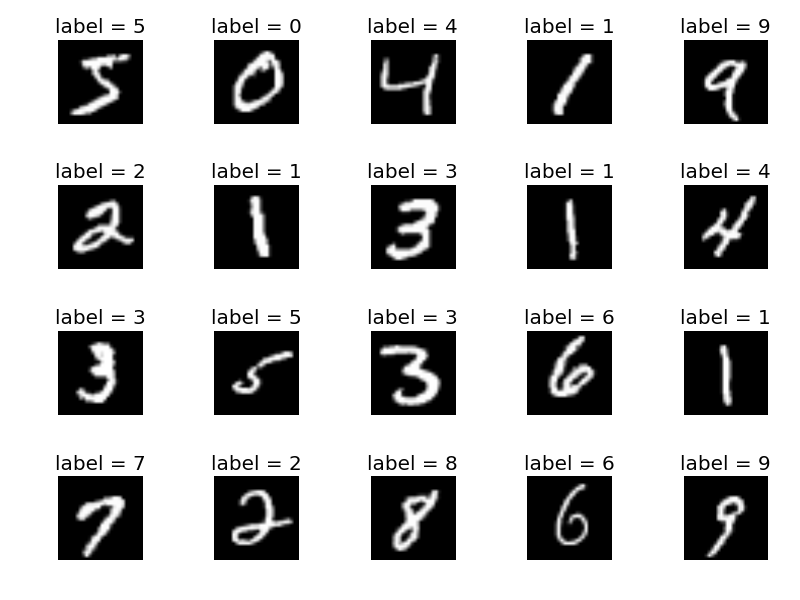
\includegraphics[width=0.5\linewidth]{images/mnist.png}
                    \caption{Some samples of MNIST dataset}
                    \label{fig:mnist}
                \end{figure}
                    
                The MNIST database (Modified National Institute of Standards and Technology database) is a large database of handwritten digits that is commonly used for training various image processing systems. The database is also widely used for training and testing in the field of machine learning. It was created by "re-mixing" the samples from NIST's original datasets. The creators felt that since NIST's training dataset was taken from American Census Bureau employees, while the testing dataset was taken from American high school students, it was not well-suited for machine learning experiments. Furthermore, the black and white images from NIST were normalized to fit into a $28 \times 28$ pixel bounding box and anti-aliased, which introduced grayscale levels. I have used $10\%$ of this dataset due to limitation of computation power and time.

            \item \textbf{Training neural network}

                Next step is to train a neural network on whom white-box attack is to be performed. I have trained a neural network with one hidden layer having $20$ neurons and one output layer having $10$ neurons. So the structure of network is $784 - [20] - 10$. The trained network performs well in test dataset. 	

            \item \textbf{Generating adversarial image}

                In this step we will use back propagation with modified error function on already trained neural network. During this process, neural network's weights are not learnable parameters, but inputs are learnable. At the beginning a random sample from dataset is fed to trained neural network. At each iteration, algorithm make relevant modifications to this input such that network make misclassification with less visual modifications on actual image.

        \end{enumerate}

    \subsection{Generated adversarial images and results}

        \Cref{fig:generated} shows some of the generated adversarial images using steps mentioned is \cref{sec:targetedattack}. All but one generated images were clearly successful in fooling trained neural network. \Cref{fig:generated} (\subref{fig:sfig4}) shows a random sample of $6$ digit with it's corresponding generated adversarial image. The trained neural network was $89\%$ confident that figure in right is $6$, but the network is $37\%$ confident that image in left is $6$. The confidence of network decreases in case of adversarial image, thus it can be concluded that all of the shown images were successful in fooling a trained neural network. 

        \begin{figure}[htbp]
            \begin{subfigure}{.5\textwidth}
                \centering
                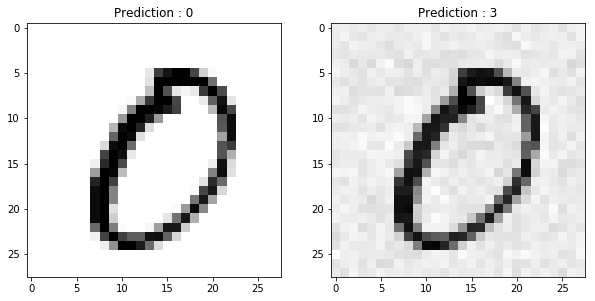
\includegraphics[width=\linewidth]{images/adversarial1.png}
                \caption{ }
                \label{fig:sfig1}
            \end{subfigure}
            \begin{subfigure}{.5\textwidth}
                \centering
                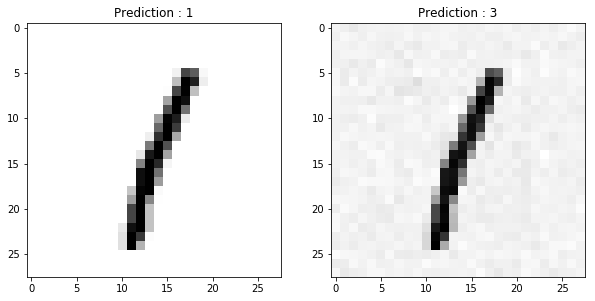
\includegraphics[width=\linewidth]{images/adversarial2.png}
                \caption{ }
                \label{fig:sfig2}
            \end{subfigure}
            \begin{subfigure}{.5\textwidth}
                \centering
                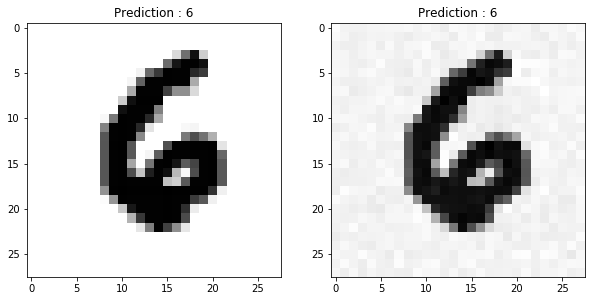
\includegraphics[width=\linewidth]{images/adversarial3.png}
                \caption{ }
                \label{fig:sfig3}
            \end{subfigure}
            \begin{subfigure}{.5\textwidth}
                \centering
                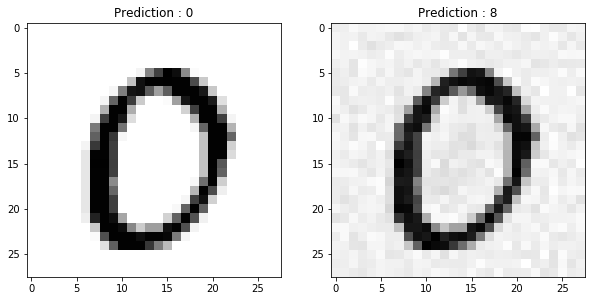
\includegraphics[width=\linewidth]{images/adversarial4.png}
                \caption{ }
                \label{fig:sfig4}
            \end{subfigure}
            \caption{Left side image is actual image from dataset and right side image is generated adversarial image}
            \label{fig:generated}
        \end{figure}
